\documentclass[12pt]{article}
\usepackage[paper=a4paper,left=30mm,right=30mm,top=35mm,bottom =35mm]{geometry}
\usepackage[utf8]{inputenc}
\usepackage[T1]{fontenc}
\usepackage{stmaryrd}
\usepackage{setspace}
\usepackage{mathrsfs}
\usepackage[ngerman]{babel}
\usepackage{amssymb}
\usepackage{amsmath}
\usepackage{fancyhdr}
\usepackage[dvips,unicode,colorlinks,linkcolor=black]{hyperref} 
\usepackage{graphicx}
\usepackage{float}
\usepackage{listings}

\pagestyle{fancy}
\lfoot{}
\rfoot{Paul Kremser, Tobias Grussenmeyer}
\cfoot{\thepage}
\fancyhead[L]{FPII Versuch: Laserspektroskopie}
\renewcommand{\headrulewidth}{0.6pt}
\renewcommand{\footrulewidth}{0.6pt}
\setlength{\headheight}{30pt}
\setlength{\parindent}{0pt}
% Für die Wahl der Schriftart
\newcommand{\changefont}[3]{
\fontfamily{#1} \fontseries{#2} \fontshape{#3} \selectfont}
%\renewcommand{\vec}[1]{\mathbf{#1}}
\renewcommand*\vec[1]{{\mbox{\boldmath\ensuremath{#1}}}}

\lstset{
	basicstyle=\ttfamily\scriptsize\mdseries,
	keywordstyle=\bfseries\color{black},
	identifierstyle=,
	commentstyle=\color{black},	
	stringstyle=\itshape\color{black},
	numbers=left,
	numberstyle=\tiny,
	stepnumber=1,
	breaklines=true,
	frame=none,
	showstringspaces=false,
	tabsize=4,
	backgroundcolor=\color{white},
	captionpos=b,
	float=htbp,
	frame=tlrb
%	extendedchars=true
}

\begin{document}
% keine Hurenkinder und Schusterjungen
\clubpenalty = 10000
\widowpenalty = 10000 
\displaywidowpenalty = 10000

\onehalfspacing
% Schriftart
\changefont{ptm}{m}{n} 

\begin{titlepage}
\author{Paul Kremser, Tobias Grussenmeyer}
\title{Versuch: Laserspektroskopie}
\date{Versuchsdurchführung: 30. März bis 2.April 2010} 
\maketitle
\thispagestyle{empty}
\end{titlepage}
%Leider schafften wir nur einen geringen Teil der gestellten Aufgaben. Ein wichtiger Teil unserer Messdataen, der des 
%letzten Tages unserer Messungen, ging verloren. Aufgrund eines Feiertages hatten wir desweiteren nur vier von fünf Möglichen Tagen zur Verfügung.

\tableofcontents
\thispagestyle{empty}
\newpage
\pagenumbering{arabic}
\section{Überblick}
In diesem Versuch soll das Prinzip der Laserspektroskopie verstanden und an einem Beispiel angewandt werden. Zusätzlich sollen Messungen zur Polarisation von
Licht und Magnetoptik gemacht werden.
Unter Laserspektroskopie versteht man verschiedene Verfahren zur Spektroskopie, in denen Laser zur Untersuchung von atomaren oder molekularen Spektren eingesetzt werden. 
In unserem Versuch wird das zu untersuchende Atom ($^{85}Rb$ und $^{87}Rb$) durch Lasereinstrahlung von einem unteren auf ein höheres Energieniveau gehoben.
Dadurch kommt es beim variieren der Laserfrequenz zu Absorptionsmaxima die mit einem Detektor gemessen werden können.
\newpage
\section{Aufgabenstellung}
\begin{itemize}
 \item Der Laser
  \begin{itemize}
   \item Bestimme die Laserschwelle 
   \item Nimm für drei Widerstände eine Spannungskurve auf
  \end{itemize}
 \item Resonator und Frequenzmodulation
  \begin{itemize}
   \item Bestimme den freien Spektralbereich $\Delta f_{FSR}$ des Resonators
   \item Aus $\Delta f_{FSR}$ die Länge des Resonators
   \item Die Finesse F des Resonators
   \item Miss die Strom-Frequenz Charakteristik der Laserdiode
   \item Charakterisiere die Frequenzmodulation
  \end{itemize}
 \item Dopplerverbreiterte Spektroskopie
  \begin{itemize}
   \item Scanne die vier Linien mit und ohne Mathe-Einheit
   \item Bestimme die Halbwertsbreiten der Linien und vergleiche sie mit dem theoretischen Wert
   \item Bestimme den Abstand der Linien
   \item Bestimme den Absorbtionsquerschnitt der vier Linien
   \item Beobachte qualitativ das Fluoreszenzsignal
  \end{itemize}
 \item Dopplerfreie Spektroskopie
  \begin{itemize}
   \item Ordne die Lambdips und Crossover-Resonanzen anhand des Termschemas von Rubidium den optischen Übergängen zu!
   \item Bestimme für beide Isotope die Hyperfeinstruktur des Grundzustandes!
   \item Miss für beide Isotope die Hyperfeinstruktur des angeregten Zustandes $5^2P_{\frac{3}{2}}$!
   \item Bestimme den Absorbtionsquerschnitt der vier Linien
   \item Beobachte qualitativ das Fluoreszenzsignal
  \end{itemize}
 \item Frequenzmodulationspektroskopie
  \begin{itemize}
   \item Frequenzmodulation des Resonators
  \begin{itemize}
   \item Vergleiche das FM-Signal mit dem DC-Signal aus der schnellen Photodiode
   \item Bestimme die Phasenverschiebung bei der das Signal invertiert erscheint
   \item Finde eine Phasenverschiebung, bei der man die Ableitung des Transmissionssignals sieht
  \end{itemize}
   \item FM-Spektroskopie an der Zelle
  \begin{itemize}
   \item Versuche, die Hyperfeinstruktur von Rubidium noch genauer auszumessen
  \end{itemize}
  \end{itemize}
  \item Messungen zur Polarisation von Licht
  \item Messungen zur Magnetoptik
\end{itemize}
\newpage

\section{Theoretische Grundlagen}
Hier soll ein Einblick in die theoretischen Grundlagen gegeben werden.
\subsection{Der Laser}
Die Abkürzung LASER steht für "Light Amplification by stimulated Emision of Radiation". Es handelt sich also um einen licht verstärkenden Effekt, der auf stimulierter Emission von Strahlung beruht. Trotz den zahlreichen Realisierungen ist das physikalische Prinzip eines jeden Lasers immer das Gleiche, es beruht auf einer Besetzungsinversion und stimulierter Emission. Des weiteren benötigt man zur Erzeugung von Laserlicht einen optischen Resonator. Um die Vorgänge beim lasen zu verstehen muss man also zunächst auf das Prinzip der Besetzungsinversion eingehen.

\subsubsection{Besetzungsinversion}
Von einer Besetzungsinversion spricht man wenn ein angeregter Zustand eines Systems stärker besetzt ist ist als ein energetisch niedrig gelegener. Es handelt sich also um eine signifikante Abweichung von der thermischen Besetzungsverteilung der Zustände in einem sogenannten aktiven Medium. Dies ist nur mit einem physikalischen Trick technisch zu realisieren.
Im folgenden sollen $Z_g$ und $Z_a$ die Zustände invertierter Besetzung mit der Energiebeziehung $E_{Z_g}<E{Z_a}$ sein.
Man erreicht Besetzungsinversion, wenn der Grundzustand $Z_g$ schnell relaxiert und die Lebensdauer kürzer ist als die durch spontane Emission bestimmte Lebensdauer des angeregten  Zustands $Z_a$. $Z_g$ muss schnell entleert werden, damit die Besetzungsinversion erhalten bleibt. Dagegen muss $Z_a$ langlebig sein, damit die Besetzung nicht durch spontane Emission soweit reduziert wird, dass die Inversion wieder ausgeglichen wird. Um nun $Z_a$ langfristig zu befüllen wird Energie mittels optischem Pumpen in das System geführt. Wird in dieses System nun Licht der Energie $E_{Z_a}-E_{Z_g}$ eingestrahlt, so kommt es zu stimulierter Emission.\\
Es existieren wie erwähnt viele technische Umsetzungen des Lasers, wir verwenden einen Halbleiderdiodenlaser.
Um eine Konzentration der induzierten Emission auf wenige Moden zu erreichen braucht man des weiteren einen optischen Resonator.

\subsubsection{Optischer Resonator}
Ein optischer Resonator ist eine Anordnung von Spiegeln, die dazu dient, Licht möglichst oft hin und her zu reflektieren. Aufgrund von Interferenz bildet sich im Resonator dann eine stehende Welle, wenn die optische Weglänge des Resonators ein Vielfaches der halben Wellenlänge des eingestrahlten Lichts beträgt. In diesem Versuch kommen zwei Resonatoren zum Einsatz. Der erste befindet sich direkt hinter dem Laser, er bildet mit der Diode eine sogenannte Litrow-Anordnung.
\subsubsection{Litrow-Anordnung}
In dieser Anordnung reflektiert man einen Teil des von der Laserdiode emittierten Lichts wieder in sich zurück. Dies geschieht mit einem Reflexionsgitter und einem Kollimator, der zwischen Laserdiode und Reflexionsgitter sitzt (Abb. \ref{litrow}). Je nach Position des Reflexionsgitters wird eine andere Wellenlänge in die Laserdiode reflektiert und verstärkt. Für die verstärkte Wellenlänge erhält man in Abhängigkeit des Winkels
\begin{align}
\label{litrowpeak}
 2d sin(\alpha) = \lambda.
\end{align}
\begin{figure}[H]
 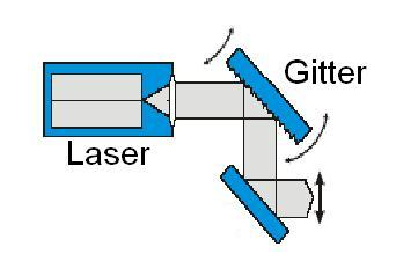
\includegraphics[width=0.9\linewidth]{pictures/litrow.eps}
 \caption{Litrow-Anordnung}
 \label{litrow}
\end{figure}
Diese Anordnung wird im Versuch benutzt um einen möglich großen modensprungfreien Bereich zu erreichen. Ein Modensprung ist ein Sprung im Transmissionsspektrum des Resonators. Er entsteht dadurch das gerade eine andere Mode in besser in den Resonator passt als die zu stabil haltende. Wir stimmen in unserem Versuch den Winkel der Litrow-Anordnung gemeinsam mit dem Laserdiodenstrom durch. Dadurch erhalten wir einen sehr viel größeren modensprungfreien Bereich also ohne Variation des Gitters. Dieses Verfahren nennt sich Feed-Vorward.
\subsubsection{Spiegel-Resonator}
\begin{figure}[H]
 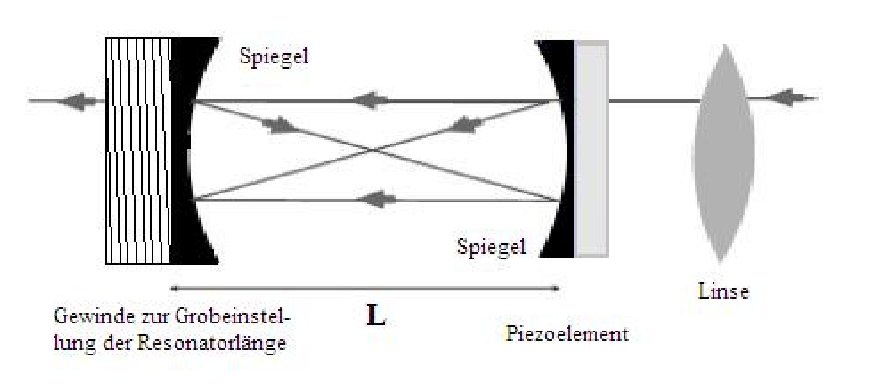
\includegraphics[width=0.9\linewidth]{pictures/cavity.eps}
 \caption{Aufbau des Spiegel-Resonators}
 \label{cavity}
\end{figure}
Der zweite Resonator in diesem Versuch ist ein sogenannter Spiegel-Resonator. Ein Spiegel-Resonator  besteht aus zwei auf der optischen Achse liegenden,
teildurchlässigen Spiegeln $S_1$ und $S_2$ im Abstand L (Abb. \ref{cavity}). Ein Resonator heißt optisch stabil, wenn ein paraxialer Lichtstrahl im Resonator
auch nach vielen Reflexionen an den Spiegeln den Resonator nicht verlässt. Wir verwenden in diesem Versuch einen konfokalen Resonator, weil er auch bei kleinen Längenänderung stabil bleibt. Die Krümmungsradien $R_1$ und $R_2$ der beiden Spiegel entsprechen in diesem Fall genau der Länge L des Resonators, es gilt $R1 =R2 = L$. Beim konfokalen Resonator beträgt der Gangunterschied zwischen durchlaufendem und reflektiertem Strahl $4L$. Es kommt zu konstruktiver Interferenz, wenn dieser Gangunterschied gerade $m\lambda$  beträgt. Daraus folgt für die Frequenzen der Transmissionslinien:
\begin{align}
\label{cavityfreq}
 f_m = \frac{mc}{4Ln}\hspace{15pt}\textnormal{ mit Brechungsindex }n\textnormal{ und } m \in \mathbb N
\end{align}
\begin{figure}[H]
 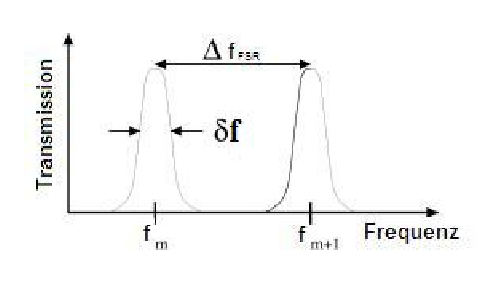
\includegraphics[width=0.9\linewidth]{pictures/cavitypeaks.eps}
 \caption{Schematischer Verlauf der Resonator-Transmissionslinien}
 \label{cavitypeaks}
\end{figure}
Der Abstand zweier Transmissionslinien (Abb. \ref{cavitypeaks}) wird als freier Spektralbereich ($\Delta f_{FSR}$) des Resonators bezeichnet. Mit Formel \ref{cavityfreq} erhält man
\begin{align}
\label{freespecrange}
 \Delta f_{FSR} = f_{m+1}-f_{m} = \frac{c}{4Ln}
\end{align}
 
Durch Reflexionsverluste an den Spiegeln haben die Linien eine endliche Halbwertsbreite $\delta f$. Ein Maß für die Anzahl der Umläufe eines Photons im Resonator stellt die Finesse $F$ des Resonators dar. Sie hängt direkt von der Reflektivität der Spiegel ab und berechnet sich zu Quotient aus freiem Spektralbereich und Halbwertsbreite
\begin{align}
\label{finesse}
 \Delta F  = \frac{\Delta f_{FSR}}{\delta f}
\end{align}
\subsection{Spektroskopie}
In unserem Versuch sollen die $D2$-Linien von zwei Rubidiumisotopen untersucht werden. Rubidium (Rb) ist ein Alkalimetall, d.h. es besitzt ein einzelnes Elektron in seiner Außenschale und hat somit ein wasserstoffähnliches Termschema(Abb \ref{term}. Es existieren zwei Isotope ($^{85}Rb$ und $^{87}Rb$) und es kommt in der Natur nicht ungebunden vor. $^{85}Rb$ ist ein stabiles Isotop, $^{87}Rb$ zerfällt sehr langsam.
\begin{figure}[H]
 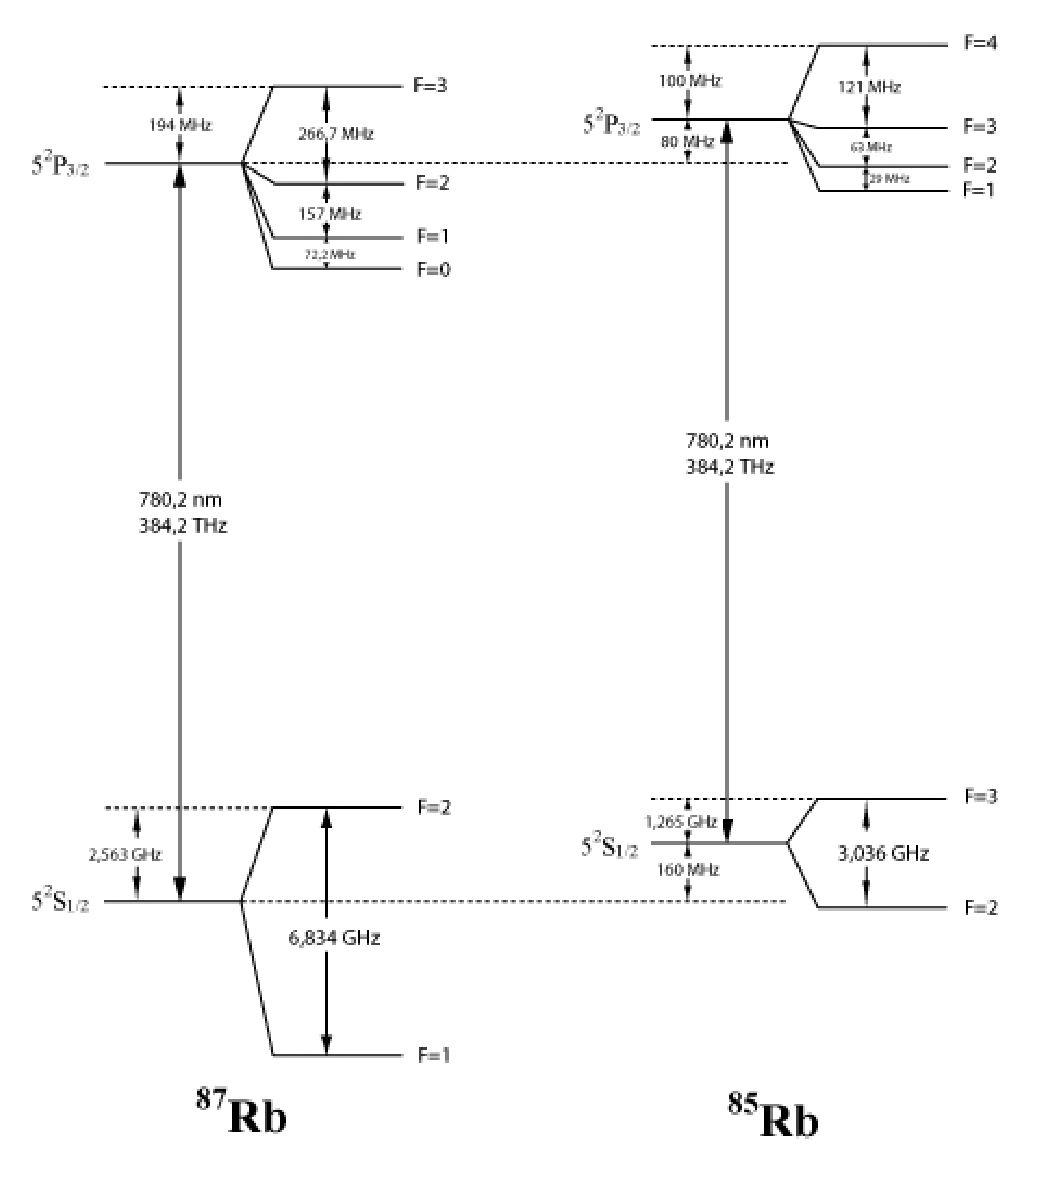
\includegraphics[width=0.9\linewidth]{pictures/term.eps}
 \caption{Termschema der $D2$-Linie von Rubidium}
 \label{term}
\end{figure}

\subsubsection{Feinstrukturaufspaltung}
Die Feinstruktur ist eine Folge der Kopplung zwischen Bahndrehimpuls $L$ des äußeren Elektrons mit seinem Spin $S$.
Der elektronische Gesamtdrehimpuls resultiert dann zu:
\begin{align}
 J = L + S
\end{align}
wobei $J$ halbzahlige Werte zwischen $|L-S|$ und $|L+S|$ annehmen kann.
Die beiden verwendeten Rubidiumisotope haben im Grundzustand $J = \frac{1}{2}$ ($L = 0$, $S = \frac{1}{2}$) und im angeregten Zustand $J = \frac{1}{2}$ bzw. $J = \frac{3}{2}$. Bei dem Übergang von $L = 0$ nach $L = 1$ spricht man von der $D$-Linie. Diese spaltet also in zwei Komponenten, die $D_1$- und die $D_2$-Linie auf. Wir untersuchen nur die $D_2$-Linie.

\subsubsection{Hyperfeinstrukturaufspaltung}
Die Hyperfeinstrukturaufspaltung resultiert aus der Kopplung des kernmagnetischen Moments $\mu_I$ mit dem am Kernort durch die Hüllenelektronen erzeugten Magnetfeld $B_J$.
Durch die Kopplung ist der Gesamtdrehimpuls $\vec{F}$, der die Summe aus Hüllendrehimpuls $\vec{J}$ und Kernspin $\vec{I}$ ist, gequantelt:
\begin{align*}
 \left|\vec{F}\right| = \hbar \sqrt{F(F+1)}
\end{align*}
Die Quantenzahl $F$ nimmt in ganzzahligen Schritten die Werte von $-I$ bis $I$ an.
\subsubsection{Linienverbreiterung}
\begin{itemize}
 \item \textbf{natürliche Linienbreite} \\
    Wegen der Heisenbergschen Unschärferelation für Energie $E$ und Zeit $t$:
    \begin{align*}
    \Delta E \Delta t \geq \hbar
    \end{align*}
    verursacht die endliche Lebensdauer $\tau$ angeregter Zustände eine natürliche Linienbreite $\Delta f_N$.
    \begin{align}
    \label{natbreite}
    \Delta f_N  = \frac{\Delta E}{h} = \frac{1}{2 \pi \tau}
    \end{align}
    Der Zustand $5^2P_{\frac{3}{2}}$ hat (bei beiden Isotopen des verwendeten Rubidiums) eine Lebensdauer von $\tau =26,5 ns$
    Die natürliche Linienbreite der Rb-Linien beträgt demnach $\Delta f_N \approx 6 Mhz$
 \item \textbf{Dopplerverbreiterung} \\
    Die Atome in der Rubidiumzelle befinden sich in einem thermischen Gleichgewicht, sie bewegen sich also. Daher erscheinen die Spektrallinien dopplerverbreitert. Es lässt sich leicht zeigen das für die vollen Halbwertsbreiten der Linien $\Delta f_{FWHM}$dann gilt:
    \begin{align}
    \label{FWHM}
     \Delta f_{FWHM} = \frac{1}{\lambda} \sqrt{\frac{8 k_B T ln 2}{m}}
    \end{align}
    Dabei ist $k_B$ die Boltzmannkonstante, $m$ die Masse und $\lambda$ die Übergangswellenlänge.
Für Zimmertemperatur und Rubidium erwartet man also eine Halbwertsbreite von $Delta f_{FWHM} \approx 500 GHz$
\end{itemize}

\subsubsection{Absorptionsquerschnitt}
Der Absorptionsquerschnitt ist in unserem Fall ein Maß für die Fläche die der Laserstrahl beim durchlaufen der Zelle sieht.
Dieser lässt sich mit dem Lambert-Beer'schen Gesetz 
\begin{align}
 I(d) = I(0) e^{-n \sigma d}
 \label{lambert}
\end{align}
mit Teilchendichte $n$, Schichtdicke $d$ und Absorptionsquerschnitt $\sigma$
für ein Zwei-Niveau-System näherungsweise bestimmen zu:
\begin{align}
 \sigma_0 \approx \frac{\lambda^2}{2\pi}.
\end{align}
Da in unserem Fall die Atome aber nicht alle Licht mit der selben Frequenz sehen muss man $\sigma_0$ noch mit dem Faktor $\frac{\Delta f_N}{\Delta f_D}$:
\begin{align}
 \sigma \approx \sigma_0 \frac{\Delta f_N}{\Delta f_D} \approx \frac{\lambda^2}{2\pi}\frac{\Delta f_N}{\Delta f_D}
\end{align}

\subsubsection{Dopplerverbreiterte Spektroskopie}
Wie der Name schon verrät spektroskopiert man in der dopplerverbreiterten Spektroskopie Linien von Übergängen welche
dopplerverbreitert sind. In unserem Versuch wird hier die Transmission der Linien von Rubidium beobachtet. Durch die große
Linienbreite lässt sich mit Hilfe der dopplerverbreiterten Spektroskopie bei Rubidium nur die Hyperfeinstruktur des Grundzustands aber nicht die
des angeregten Zustands auflösen. Im Wesentlichen wird bei dieser Spektroskopie Licht auf das zu untersuchende Medium gestrahlt und hinter dem Medium die Intensität gemessen. Durch Variation der Wellenlänge des eingestrahlten Lichts lassen sich verschiedene Zustände im Medium anregen: Entspricht die eingestrahlte Wellenlänge gerade der eines Übergangs im Medium, so wird dieser Übergang angeregt und somit das einfallende Licht absorbiert. Dies bedeutet wiederum, dass die hinter dem Medium gemessene Intensität abnimmt. Dieses Verfahren nennt man auch Transmissionsspektroskopie.

\subsubsection{Dopplerfreie Spektroskopie}
Durch eine geschickte Anordnung des Versuchsaufbaus lässt Spektroskopie auch dopplerfrei durchführen.
Hierzu lässt man das zu spektroskopierende Medium von zwei Strahlen durchlaufen welche sich im Medium überlappen aber in entgegengesetzter Richtung verlaufen. Oft wird der Strahl nach dem ersten Durchlauf einfach wieder in sich zurück reflektiert. Bei dieser Anordnung gibt es zwei mögliche Situationen:
\begin{itemize}
 \item Die Wellenlänge des eingestrahlten Lichts entspricht gerade einem Übergang der Atome die ruhen.
 \item Die Wellenlänge entspricht gerade nicht dem Übergang der ruhenden Atome.
\end{itemize}
Im ersten Fall werden durch den ersten Strahl, auch Sättigungsstrahl genannt, gerade die Atome in das höhere Niveau des Übergangs angeregt welche ruhen. Für den rücklaufenden, zweiten Strahl, auch Abfragestrahl genannt, erscheint das Medium transparent, da sich bei ausreichender Intensität des Sättigungsstrahl die meisten verfügbaren ruhenden Atome schon im angeregten Zustand befinden. Im Zweiten Fall dagegen, besteht die Übereinstimmung von Wellenlänge mit Übergang der einen Strahlrichtung gerade aus der entgegengesetzten Geschwindigkeitsklasse der anderen Strahlrichtung. Somit ist in diesem Fall keine Transparenz des Mediums für den Rücklaufenden Strahl gegeben. Die bei dieser Anordnung beobachteten Peaks nennt man \textbf{Lambdips}. Hat das Medium mehrere Übergänge und ist deren Abstand kleiner als die maximal auftretende Dopplerverschiebung, so entstehen bei der dopplerfreien Spektroskopie auch noch weitere Peaks, die sogenannten \textbf{crossover Resonanzen}. Diese liegen immer genau zwischen zwei Lambdips. Liegt die eingestrahlte Wellenlänge genau zwischen zwei Übergängen, so existiert eine Geschwindigkeitsklasse die für den einen Übergang gerade dem Sättigungsstrahl entspricht und für den anderen Übergang dem Abfragestrahl. Da der Sättigungsstrahl diese Geschwindigkeitsklasse somit in den einen angeregten Zustand anhebt, erscheint das Medium für den Abfragestrahl (dieser würde ja gerade die selbe Geschwindigkeitsklasse, also die selben Atome in den anderen Zustand anheben) transparent. Mit der dopplerfreien Spektroskopie lässt sich an Rubidium auch die Hyperfeinstruktur des angeregten Zustands auflösen.

\section{Versuchsaufbau}
Der Versuchsaufbau besteht aus diversen Optischen und Elektronischen Komponenten die im folgenden Erläutert werden.
Die Beschreibung der konkreten Verwendung für die einzelnen Versuchsteile erfolgt anschließend.
\subsection{Optik}
Grundsätzlich werden alle optischen Elemente auf eine Metallplatte mit einem Lochraster geschraubt. Hierdurch kann ein ungewolltes verschieben der Elemente verhindert werden. Auf dieser Platte befindet sich bereits der Laser zusammen mit seinem Resonator, außerdem ein Strahlheber welcher den Laserstrahl auf eine angenehme Arbeitshöhe hebt. Zudem befinden sich ebenfalls ein Prismenpaar, welches den Strahl möglichst Kreisförmig machen soll, und ein optischer Isolator (lässt den Strahl nur in eine Richtung durch). Für die verschiedenen Versuchsteile stehen nun folgende optische Elemente zur Verfügung:
\begin{itemize}
 \item diverse Spiegel
 \item $\frac{\lambda}{2}$-Plättchen
 \item $\frac{\lambda}{4}$-Plättchen
 \item Polarizing Beam Splitter
 \item zwei langsame und eine schnelle Photodiode
 \item Cavity (externer optischer Resonator)
 \item Rubidiumzelle
\end{itemize}
\newpage 
\subsubsection{Leistung-Laserdiodenstrom-Kennlinie}
Für die Aufnahme der Photodiodenkennlinien werden die optischen Elemente wie in Abbildung \ref{skizze-pd} angeordnet.
Über die Kombination aus $\frac{\lambda}{2}$-Plättchen und PBS kann die auf die Fotodiode treffende Intensität verändert werden. Somit kann man an diesem Aufbau auch gleich das verhalten des Beamsplitters studieren.
\begin{figure}[H]
 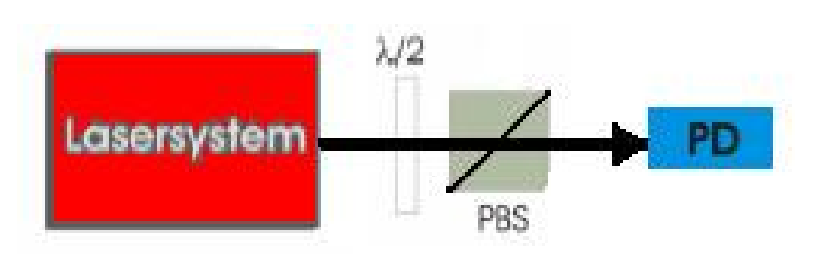
\includegraphics[width=0.9\linewidth]{pictures/eichung_der_photodiode.eps}
 \caption{Aufbau Photodiodenkennlinien}
 \label{skizze-pd}
\end{figure}
\newpage
\subsubsection{Messungen am Resonator}
Für die Messungen am Resonator ``Cavity scannen'' wird der Aufbau wie in Abbildung \ref{skizze-cavity} verwendet. Wichtig ist hierbei, dass zwei Spiegel verwendet werden, da es sonst nicht möglich ist den Strahl parallel durch den Resonator laufen zu lassen. Hier wird ein sogenannter ``Beam Walk'' durchgeführt, im wesentlichen wird abwechselnd an den beiden Spiegeln gedreht bis das Signal der Photodiode maximal ist. Die für den ``Beam Walk'' geeignete Vorgehensweise ist gut in der Versuchsanleitung beschrieben.
\begin{figure}[H]
 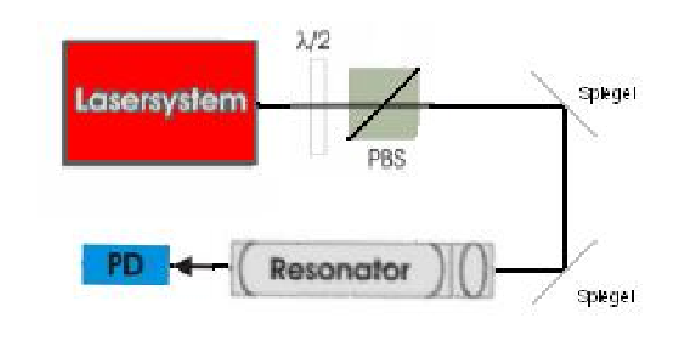
\includegraphics[width=0.9\linewidth]{pictures/experiment_am_resonator.eps}
 \caption{Aufbau Cavity scannen}
 \label{skizze-cavity}
\end{figure}
\newpage
\subsubsection{Dopplerverbreiterte Spektroskopie}
Für die dopplerverbreiterte Spektroskopie am Rubidium wird nun auch noch die Rubidiumzelle in den Strahlengang eingebracht.
Diese wird leicht schräg zum Strahlengang positioniert um die an den Endflächen der Zelle auftretenden Reflexionen nicht in den Strahl zurück zu führen. Der Aufbau ist Schematisch in Abbildung \ref{skizze-dopplerbreit}
\begin{figure}[H]
 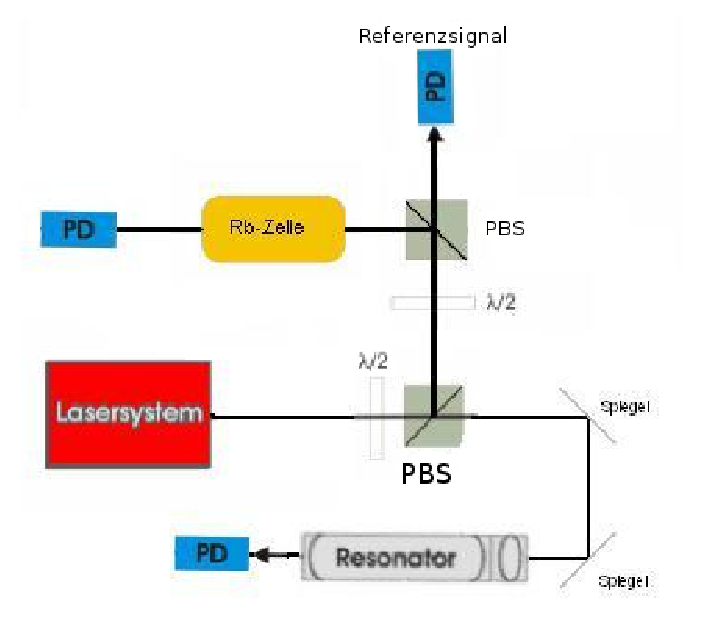
\includegraphics[width=0.9\linewidth]{pictures/aufbau_doppler.eps}
 \caption{Aufbau dopplerverbreiterte Spektroskopie}
 \label{skizze-dopplerbreit}
\end{figure}
\newpage
\subsubsection{Dopplerfreie Spektroskopie}
Bei der dopplerfreien Spektroskopie wird fast der selbe Aufbau wie für die dopplerverbreiterte verwendet. Es wird lediglich die Photodiode hinter der Rubidiumzelle durch einen Spiegel und ein $\frac{\lambda}{4}$-Plättchen ersetzt und hinter dem zweiten PBS platziert. Siehe Abbildung \ref{skizze-dopplerfrei}
\begin{figure}[H]
 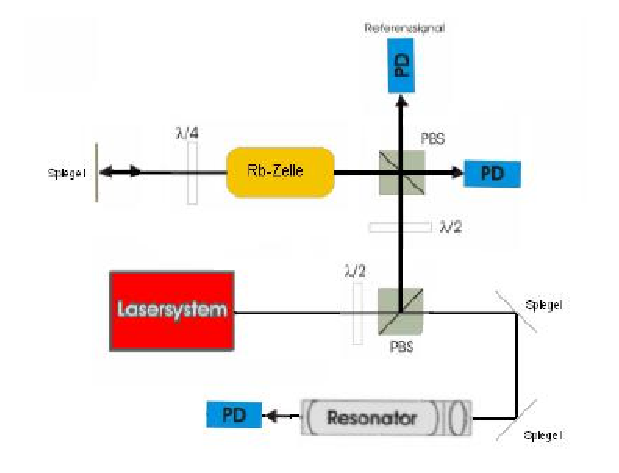
\includegraphics[width=0.9\linewidth]{pictures/aufbau_dopplerfrei.eps}
 \caption{Aufbau dopplerfreie Spektroskopie}
 \label{skizze-dopplerfrei}
\end{figure}
\newpage

\section{Auswertung}
\subsection{Der Laser}
Zunächst untersuchten wir die Laserschwelle grob mit der Infrarotkarte. Wir sahen ab $I_{Laser} \approx 20 mA$ ein einsetzen der Strahlung.
Die Photodiodenkennlinien mit den drei Widerständen sind in Abb. \ref{pdkennlinien1} und \ref{pdkennlinien2} dargestellt. Wir bestimmten daraus die Laserschwelle zu:
\begin{align*}
 I_{Laser, \Omega} = (72 \pm 2) mA. \\
\end{align*}
hierbei handelt es sich um geschätzte Ablesefehler.
\begin{figure}[H]
 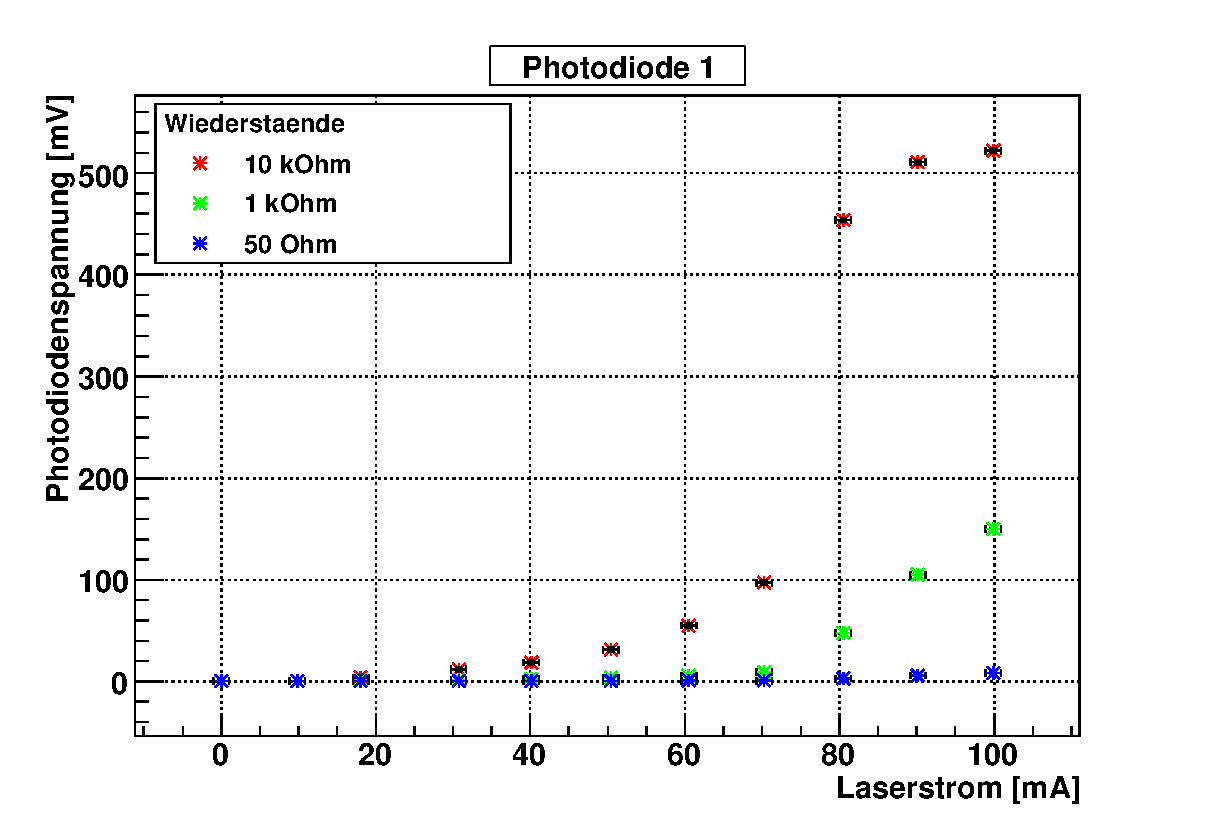
\includegraphics[width=0.9\linewidth]{pictures/pd_kenn1.eps}
 \caption{Kennlinien der passiven Photodiode 1 für die drei schaltbaren Widerstände}
 \label{pdkennlinien1}
\end{figure}
\begin{figure}[H]
 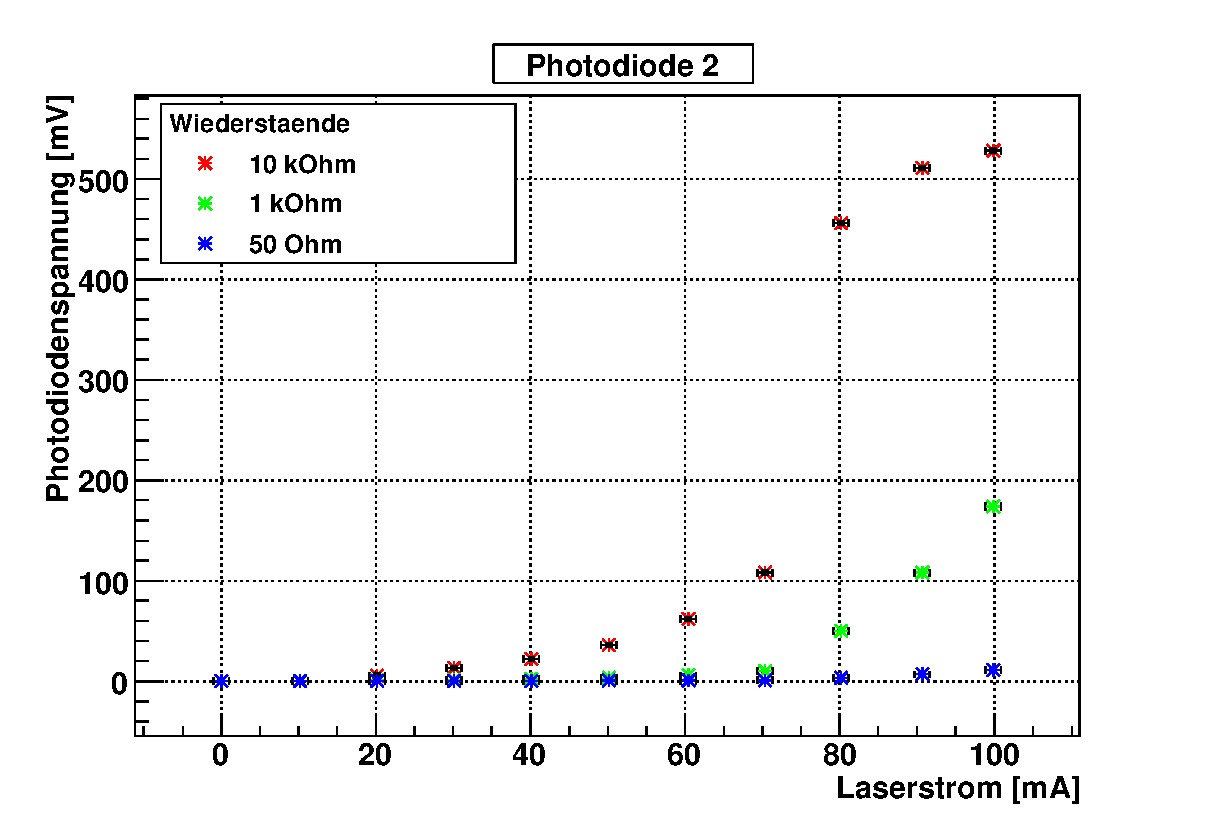
\includegraphics[width=0.9\linewidth]{pictures/pd_kenn2.eps}
 \caption{Kennlinien der passiven Photodiode 2 für die drei schaltbaren Widerstände}
 \label{pdkennlinien2}
\end{figure}

\subsection{Der Resonator}
Um den freien Spektralbereich bestimmen zu können braucht man zunächst eine Frequenzeichung. Wir modulierten also unterschiedliche Frequenzen auf die Laserfrequenz.Für die Abstände der Seitenbänder $d_{\mu s}$ und der Modulationsfrequenz $f_M$muss dann folgender Zusammenhang gelten:
\begin{align*}
 f_M = A \cdot d_{\mu s}
\end{align*} 
\begin{figure}[H]
 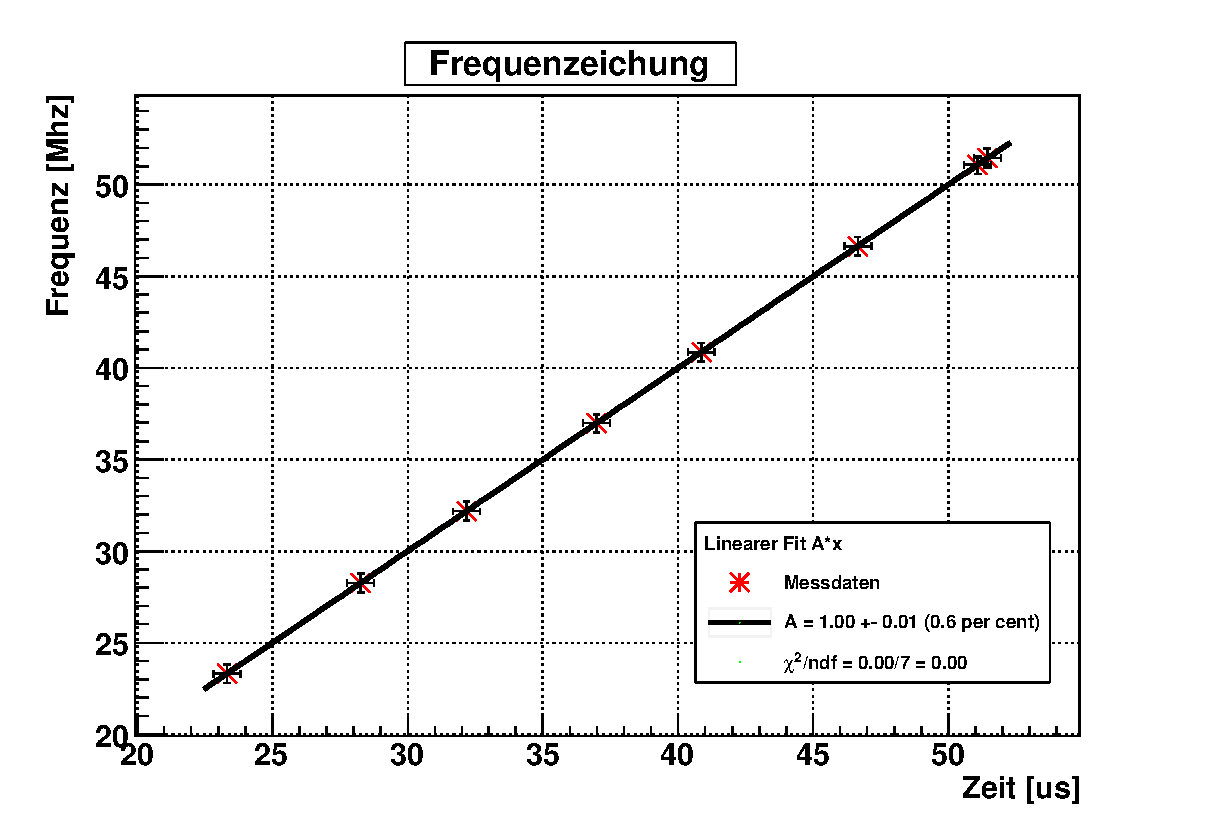
\includegraphics[width=0.9\linewidth]{pictures/eichung.eps}
 \caption{Frequenzeichung über Modulation}
 \label{eichung}
\end{figure}
in Abb. \ref{eichung} sind unsere Daten Zusammen mit dem Fit dargestellt. Die Fehler sind auch hier Ablesefehler. Wir erhielten also für $A$:
\begin{align*}
 A = (1 \pm 0,006) \frac{1}{s^2}
\end{align*} 
Wir bestimmten den freien Spektralbereich $\Delta f_{FSR}$ indem wir die Abstände $d_i$ von zwölf Resonatorpeaks mittelten. Auch hier schätzten wir während der Messung einen Fehler auf die Ablesegenauigkeiten unserer Messdaten. Aus obiger Energieeichung erhielten wir dann:
\begin{align*}
 \Delta f_{FSR} = (790\pm5) Mhz
\end{align*}
hierbei berechnete sich der Fehler nach der Gaußschen Fehlerfortpflanzung zu
\begin{align*}
 s_{\Delta f_{FSR}} = \Delta f_{FSR} \cdot \sqrt{ \left( \frac{s_A}{A} \right)^2 + \left( \frac{s_{d_i}}{d_i} \right)^2}
\end{align*}
Dieser Fehler überträgt sich nach Gaußscher Fehlerfortpflanzung auf viele nachfolgende Messungen. Dies liegt daran das dieser Wert später zur Eichung der Zeitachse genommen wird. Dabei wird ein Umrechnungsfaktor $U$ so bestimmt das $t\cdot U=f$, wenn $t$ die Zeit und $f$ die Frequenz sind. Der Fehler des Umrechnungsfaktors berechnet sich nach Gaußscher Fehlerfortpflanzung zu
\begin{align*}
 s_U = U \sqrt{ \left( \frac{s_{\Delta f_{FSR}}}{\Delta f_{FSR}} \right) ^2 + \left( \frac{s_{T_{\Delta f_{FSR}}}}{T_{\Delta f_{FSR}}} \right) ^2 }
\end{align*}
wobei $T_{\Delta f_{FSR}}$ den Fehler auf eine Zeitmessung zur Bestimmung von $\Delta f_{FSR}$ bezeichnet. Bei einigen Messungen dominierte dieser Fehler deutlich.

Weiter lässt sich über $\Delta f_{FSR} = \frac{c}{4Ln}$ auch die Länge des Resonators bestimmen. Wir erhielten
\begin{align*}
 L_{Resonator}= (9,5 \pm 0,06) cm
\end{align*}
dabei überträgt sich hier der relative Fehler von $\Delta f_{FSR}$.  \\
Weiter bestimmten wir mit dem Oszilloskop die Halbwertsbreiten $\delta f$ von fünf Resonatorpeaks und mittelten diese, um damit die Finesse $F$ des Resonators zu bestimmen. Wir erhielten 
\begin{align*}
 F = \frac{\Delta f_{FSR}}{\delta f} = ( 23,35 \pm 0,2 )
\end{align*}
hierbei berechnete sich der Fehler nach der Gaußschen Fehlerfortpflanzung zu
\begin{align*}
 s_F = F \cdot \sqrt{ \left( \frac{s_{\Delta f_{FSR}}}{\Delta f_{FSR}} \right)^2 + \left( \frac{s_{\delta f}}{\delta f} \right)^2}
\end{align*}
Leider mussten wir nach Beendigung des Versuchs feststellen das wir vergessen hatten die Piezo-Frequenz-Charakteristik zu vermessen. 
Wir charakterisierten die Frequenzmodulation und verglichen sie mit den theoretischen Werten, die Ergebnisse hiervon sind in Abb. \ref{bessel} zu sehen.
\begin{figure}[H]
 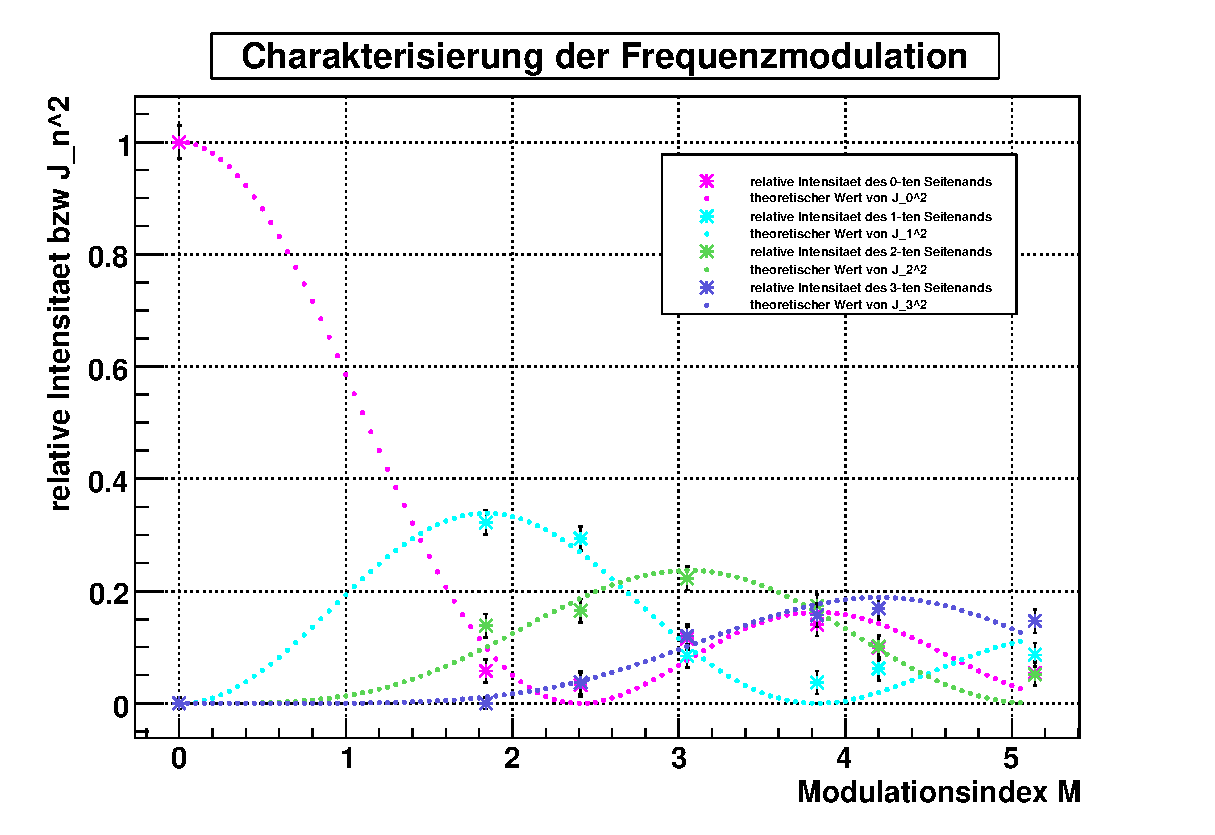
\includegraphics[width=0.9\linewidth]{pictures/modulation.eps}
 \caption{Charakterisierung der Frequenzmodulation}
 \label{bessel}
\end{figure}

\subsection{Dopplerverbreiterte Spektroskopie}
\begin{figure}[H]
 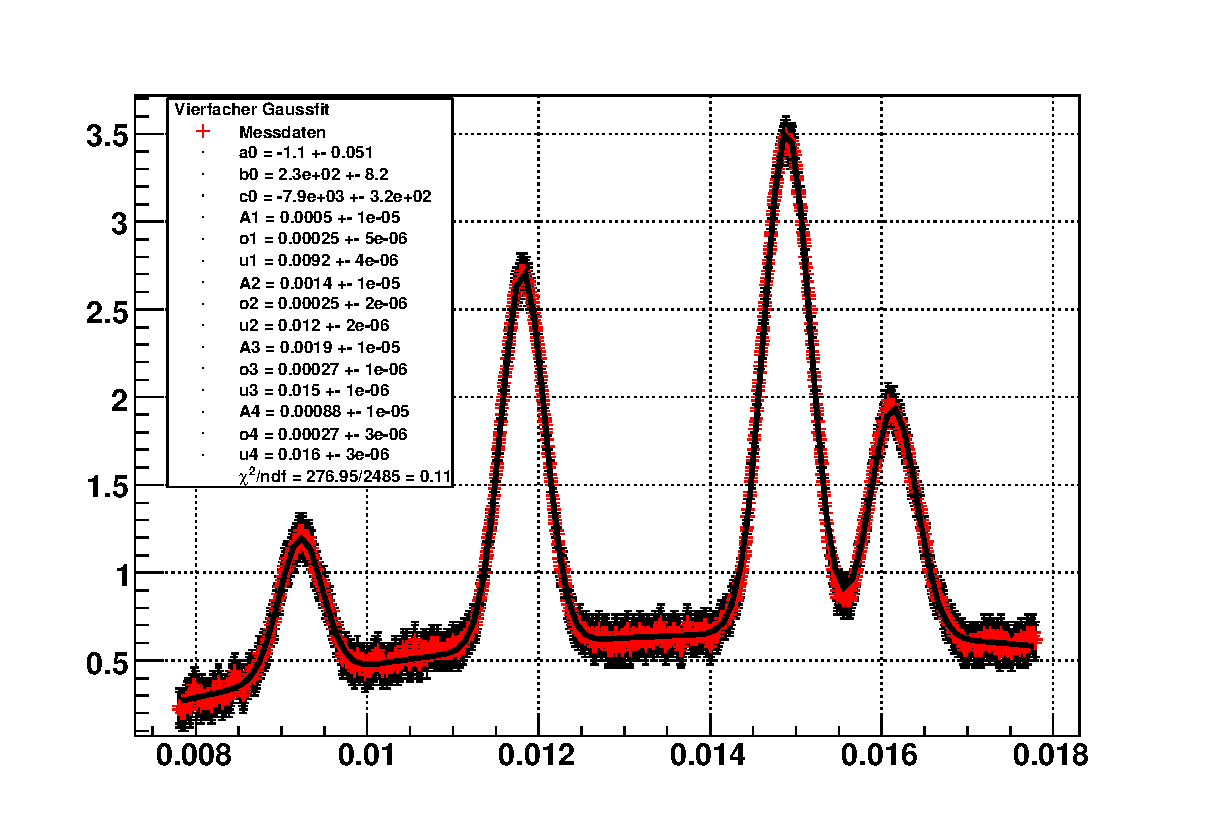
\includegraphics[width=0.9\linewidth]{pictures/doppler.eps}
 \caption{Frequenzeichung über Modulation}
 \label{doppler}
\end{figure}
\subsubsection{Linienbreite}
Wir untersuchten die vier Linien mit und ohne Mathe-Einheit, als Differenz und Quotient. Aus der Linienform der Referenzdiode und den Ergebnissen beim fitten schlossen wir, das ein eine Faltung aus vier Gaußkurven mit einem Polynom 2.Grades die Daten am besten repräsentiere. Das Ergebnis unseres Fits an ein Signal, gemessen als Quotient, ist in Abb \ref{doppler} zu sehen. Aus den Parametern der Gaußbreiten des Fits berechneten wir Die volle Halbwertsbreite in $\mu s$. Über einen mitaufgenommenen Frequenzkamm rechneten wir sie in eine Frequenzen um. Zuletzt bildeten wir das gewichtete Mittel und erhielten als Dopplerbreite $\Delta f_{FWHM}$:
\begin{align*}
 \Delta f_{FWHM} = (621 \pm 3) GHz
\end{align*}
hierbei berechnete sich der Fehler nach der Gaußschen Fehlerfortpflanzung. Die Einzelmessungen ergaben:
\begin{center}
\begin{tabular}{|l|l|l|l|l|}
\hline
Peak & 1 & 2 & 3 & 4\\
\hline
$\Delta f_{FWHM} [Mhz]$ & $596\pm12$ & $598 \pm 6$ & $633 \pm 5$ & $635 \pm 8$\\
\hline
\end{tabular}
\end{center}
\subsubsection{Abstände der Linien}
Aus den Fits in Abb \ref{doppler} erhielten wir die Schwerpunkte der Peaks. Wir ordneten sie ihren Zuständen zu. Das Ergebnis ist in Tabelle \ref{order} dargestellt. Die Abstände sind in Tabelle \ref{dist} dargestellt.

\begin{table}[H]
\begin{center}
\begin{tabular}{|l|l|l|l|l|}
\hline 
Peak & 1 & 2 & 3 & 4\\
\hline
Isotop & $^{87}Rb$ & $^{85}Rb$ & $^{85}Rb$ & $^{87}Rb$\\
$F$ of $5^2S_{\frac{1}{2}}$ & 1 & 2 & 3 & 2 \\
\hline
\end{tabular}
\end{center}
\caption{Zuordnung der Peaks}
\label{order}
\end{table}

\begin{table}[H]
\begin{center}
\begin{tabular}{|l|l|l|l|}
\hline
Peaks & 1 und 2 & 2 und 3 & 3 und 4\\
\hline
Abstand [Ghz] & $2,59 \pm 0.02$ & $3,08 \pm 0,02$ & $1,243 \pm 0,01$\\
\hline
\end{tabular}
\end{center}
\caption{Abstaende der Peaks}
\label{dist}
\end{table}


\subsubsection{Absorptionsquerschnitt}
Da der Absorptionsquerschnitt $\sigma$ direkt vom Quotient der Intensitäten vor und hinter der Zelle abhängt, konnten wir diesen mittels des Gaußparameters bestimmen. Aus Gleichung \ref{lambert} folgt nämlich
\begin{align*}
 \sigma = \frac{ln \left( \frac{I_0}{I_d} \right) }{nd} 
\end{align*}
Wir haben den Quotienten aus Spannung der Photodiode vor und hinter der Zelle gemessen, welchen wir in obige Gleichung einsetzten. Allerdings trauten wir dieser Methode trotz Offsetanpassung nicht da wir nicht sicher sein konnten das beide Detektoren Lichtsignale wirklich gleich verstärkt wiedergeben. Des weiteren hatte die Mathe-Einheit immer wieder Funktionsstörungen, weshalb wir auch hier eine Fehlerquelle dieser Methode vermuteten.
\begin{center}
\begin{tabular}{|l|l|l|l|l|}
\hline 
Peak & 1 & 2 & 3 & 4\\
\hline
$\sigma [10^{-17} m^2]$ & $4,8 \pm 0,1$ & $13,2 \pm 0,1$ & $18,7 \pm 0,1$ & $8.5 \pm 0,1$\\
\hline
\end{tabular}
\end{center}

\section{Zusammenfassung}
Begonnen hatten wir mit der Feststellung der Laserschwelle, wobei wir mit Hilfe der Photodioden einen Wert von:
\begin{align*}
 I_{Laser, \Omega} = (72 \pm 2) mA. 
\end{align*}
erhielten.\\

Anschließend hatten wir uns dem externen Resonator zugewendet und dessen freien Spektralbereich bestimmt zu:
\begin{align*}
 \Delta f_{FSR} = (790\pm5) Mhz.
\end{align*}
außerdem erhielten wir für die Finesse des Resonators:
\begin{align*}
 F = \frac{\Delta f_{FSR}}{\delta f} = ( 23,35 \pm 0,2 ).
\end{align*}
Für die Länge des Resonators haben wir:
\begin{align*}
 L_{Resonator}= (9,5 \pm 0,06) cm
\end{align*}
berechnet. Da man die genaue Position der Spiegel im Resonator von außen nicht sehen kann lies sich seine Länge nur grob messen. Hier hatten wir die Länge auf ca. $10cm$ bestimmt, wobei man hier einen Fehler von fast einem Zentimeter annehmen kann. Somit stimmen die beiden Längen gut überein.\\

Bei der dopplerfreien Spektroskopie verwendeten wir den Resonator als Frequenzlineal und konnten somit die Abstände der Peaks und deren Breiten im Rubidiumspektrum vermessen.
Die mittlere Breite der Peaks haben wir bestimmt zu:
\begin{align*}
 \Delta f_{FWHM} = (621 \pm 3.2) GHz.
\end{align*}
Die theoretische erwartete Halbwertsbreite liegt bei $\Delta f_{FWHM} \approx 500 Ghz$. Wir haben somit breitere Peaks als erwartet gemessen. Dies kann viele Ursachen haben, in erster Linie wird in dem Versuch viel Elektronik verwendet was eigentlich immer eine gaußförmige Verbreiterung bedeutet.
Die drei Abstände haben wir zu:
\begin{table}[H]
\begin{center}
\begin{tabular}{|l|l|l|l|}
\hline
Peaks & 1 und 2 & 2 und 3 & 3 und 4\\
\hline
Abstand [Ghz] & $2,59 \pm 0.02$ & $3,08 \pm 0,02$ & $1,243 \pm 0,01$\\
\hline
\end{tabular}
\end{center}
\end{table}
bestimmen können.
Aus dem Termschema von Rubidium lassen sich die theoretischen Werte ablesen zu:
\begin{table}[H]
\begin{center}
\begin{tabular}{|l|l|l|l|}
\hline
Peaks & 1 und 2 & 2 und 3 & 3 und 4\\
\hline
Abstand [Ghz] & $2,66$ & $3,036$ & $1,138$\\
\hline
\end{tabular}
\end{center}
\end{table}
Die Abweichungen der ersten beiden Werte liegen im vier bzw. drei Sigma Bereich, der dritte Wert jedoch weicht weit von der Literatur ab.\\

Für den Absorptionsquerschnitt der Linien haben wir:
\begin{center}
\begin{tabular}{|l|l|l|l|l|}
\hline 
Peak & 1 & 2 & 3 & 4\\
\hline
$\sigma [10^{-17} m^2]$ & $4,8 \pm 0,1$ & $13,2 \pm 0,1$ & $18,7 \pm 0,1$ & $8.5 \pm 0,1$\\
\hline
\end{tabular}
\end{center}
berechnet. Eine Aussage über die Qualität der Werte ist schwer da hier die Qualität der Matheeinheit eingeht und diese nicht bekannt ist (Unterschiedliche Verstärkungen der Kanäle wirken sich auf das Teilungsverhältnis aus.)\\

Leider haben wir am letzten der vier Tage die uns für den Versuch zur Verfügung standen vergessen die CF-Karte aus dem Oszilloskop auf den PC zu kopieren. Die Daten zur Dopplerfreien- und FM-Spektroskopie sind uns somit leider verloren gegangen. Dennoch konnten wir die Hyperfeinstrukturaufspaltung des Angeregten Zustands bei der Durchführung sehen und das Prinzip der Laserspektroskopie verstehen. Für die Versuchsteile zur Polarisation von Licht und Magnetooptik fehlte uns leider die Zeit weshalb wir auf eine Beschreibung verzichteten.
\section{Quelltext}
Zur Auswertung verwendeten wir das Datenanalyseframework PyRoot. Die Quelltexte sind im folgenden angehängt.

%\lstinputlisting[language=python, extendedchars=false, inputencoding=utf8]{../staebe/staebe.py}

\end{document}
